\documentclass[output=paper,colorlinks,citecolor=brown,
% hidelinks,
% showindex
]{langscibook}
\author{Heather Newell\affiliation{
Université du Québec à Montréal}\orcid{}}
\title{Tamil pronominal alternations are phonology not allomorphy}
\abstract{Abstract goes here}

%move the following commands to the "local..." files of the master project when integrating this chapter
\usepackage{tabularx}
\usepackage{langsci-basic}
\usepackage{langsci-optional}
\usepackage{langsci-gb4e}
\usepackage{multicol}
\usepackage[linguistics]{forest}

%Tikz

\usepackage{textgreek}
\usepackage{tikz}
\usepackage{pgf}
\usetikzlibrary{backgrounds, matrix, positioning}
\usepackage{tipa}

\bibliography{localbibliography}
\newcommand{\orcid}[1]{}
\pagenumbering{roman}

\IfFileExists{../localcommands.tex}{%hack to check whether this is being compiled as part of a collection or standalone
   % add all extra packages you need to load to this file
\usepackage{tabularx,multicol}
\raggedcolumns

\usepackage{url}
\urlstyle{same}

\usepackage{listings}
\lstset{basicstyle=\ttfamily,tabsize=2,breaklines=true}

\usepackage{langsci-basic}
\usepackage{langsci-optional}
\usepackage{langsci-lgr}

% Wood's chapter
\usepackage{jimsstyle}

\usepackage{subcaption}
\usepackage{color,colortbl}
\definecolor{Gray}{gray}{0.8}%to get a color for the table
\usepackage{expex}
\usepackage[linguistics]{forest}
\forestset{qtree edges/.style={for tree={parent anchor=south, child anchor=north}}}
\usepackage{graphbox}
\usepackage{leipzig}
\usepackage{multirow}
\usepackage{needspace}
\usepackage{newunicodechar}
\usepackage{pifont}
\usepackage{pgf}
\usepackage{pst-node}
\usepackage{qtree}
  \qtreecenterfalse
\usepackage{rotating}
% \usepackage{skak}
\usepackage{soul}
\usepackage{tabto}
\usepackage{textgreek}
\usepackage{tikz}
\usetikzlibrary{calc,decorations,shapes.misc,decorations.pathreplacing,arrows}
\usetikzlibrary{backgrounds, matrix, positioning}
\usetikzlibrary{}
\usetikzlibrary{}
\usepackage{tikz-qtree,tikz-qtree-compat}
\usepackage{tipa} % must be imported before linguex, but we do not use linguex here
\usepackage{todonotes}
\usepackage{tree-dvips}
\usepackage[normalem]{ulem}%for strikeout
\usepackage[Symbolsmallscale]{upgreek} 
\usepackage{verbatim}
\usepackage{xcolor}
\usepackage{xspace}
% \usepackage{xtab}

\usepackage{langsci-gb4e}

   \newcommand{\orcid}[1]{}


% pesetskycommands.tex
%ExPex stuff

\newcommand{\pexcnn}{\pex[exno={~},exnoformat={X}]}  % pexc with no examplenumber and no increment
\lingset{everygla=\normalfont,{aboveglftskip=0pt}}
\newcommand{\ptxt}[1]{#1\par}
\let\expexgla\gla
\AtBeginDocument{\let\gla\expexgla\gathertags}

%other stuff
\newunicodechar{⟶}{{\symbolfont{⟶}}}
%\newunicodechar{✓}{{\Checkmark}} % checkmark
\newunicodechar{✓}{{\ding{51}}} % checkmark
\newcommand{\gap}{\ \underline{\hspace{10pt}\phantom{x}}\ }
\newcommand{\ix}[1]{\textsubscript{\it{#1}}}  % subscript

\def\gethyperref#1{\hyperlink{#1}{\getref{#1}}}%
\def\getfullhyperref#1{\hyperlink{#1}{\getfullref{#1}}}%

\newcommand{\denote}[1]{⟦{#1}⟧}

   %% hyphenation points for line breaks
%% Normally, automatic hyphenation in LaTeX is very good
%% If a word is mis-hyphenated, add it to this file
%%
%% add information to TeX file before \begin{document} with:
%% %% hyphenation points for line breaks
%% Normally, automatic hyphenation in LaTeX is very good
%% If a word is mis-hyphenated, add it to this file
%%
%% add information to TeX file before \begin{document} with:
%% %% hyphenation points for line breaks
%% Normally, automatic hyphenation in LaTeX is very good
%% If a word is mis-hyphenated, add it to this file
%%
%% add information to TeX file before \begin{document} with:
%% \include{localhyphenation}
\hyphenation{
affri-ca-te
affri-ca-tes 
agree-ment
anaph-o-ra
an-ti-caus-a-tive
an-ti-caus-a-tives
an-te-ced-ent
Bak-er
caus-a-tive
Christo-poulos
clas-si-fi-er
claus-al
Co-lum-bia
com-ple-ment-izer
com-ple-ments
con-tin-u-a-tive
de-di-ca-ted
De-mo-cra-tas
Dor-drecht
du-ra-tive
Ex-folia-tion
ex-tra-gram-mat-ical
fi-nite-ness
ger-und
ger-unds
Gro-ninger
in-trac-ta-ble
Jap-a-nese
judg-ment
Judg-ment
Lysk-awa
Ma-khach-ka-la
Ma-rantz
Mat-thew-son
Max-Share
merg-er
Pap-u-an
Per-elts-vaig
post-ver-bal
phe-nom-e-non
pre-dic-tion
Pre-dic-tion
Rich-ards
Sa-len-ti-na
to-pic
Ya-wa-na-wa
Wil-liam-son
}

\hyphenation{
affri-ca-te
affri-ca-tes 
agree-ment
anaph-o-ra
an-ti-caus-a-tive
an-ti-caus-a-tives
an-te-ced-ent
Bak-er
caus-a-tive
Christo-poulos
clas-si-fi-er
claus-al
Co-lum-bia
com-ple-ment-izer
com-ple-ments
con-tin-u-a-tive
de-di-ca-ted
De-mo-cra-tas
Dor-drecht
du-ra-tive
Ex-folia-tion
ex-tra-gram-mat-ical
fi-nite-ness
ger-und
ger-unds
Gro-ninger
in-trac-ta-ble
Jap-a-nese
judg-ment
Judg-ment
Lysk-awa
Ma-khach-ka-la
Ma-rantz
Mat-thew-son
Max-Share
merg-er
Pap-u-an
Per-elts-vaig
post-ver-bal
phe-nom-e-non
pre-dic-tion
Pre-dic-tion
Rich-ards
Sa-len-ti-na
to-pic
Ya-wa-na-wa
Wil-liam-son
}

\hyphenation{
affri-ca-te
affri-ca-tes 
agree-ment
anaph-o-ra
an-ti-caus-a-tive
an-ti-caus-a-tives
an-te-ced-ent
Bak-er
caus-a-tive
Christo-poulos
clas-si-fi-er
claus-al
Co-lum-bia
com-ple-ment-izer
com-ple-ments
con-tin-u-a-tive
de-di-ca-ted
De-mo-cra-tas
Dor-drecht
du-ra-tive
Ex-folia-tion
ex-tra-gram-mat-ical
fi-nite-ness
ger-und
ger-unds
Gro-ninger
in-trac-ta-ble
Jap-a-nese
judg-ment
Judg-ment
Lysk-awa
Ma-khach-ka-la
Ma-rantz
Mat-thew-son
Max-Share
merg-er
Pap-u-an
Per-elts-vaig
post-ver-bal
phe-nom-e-non
pre-dic-tion
Pre-dic-tion
Rich-ards
Sa-len-ti-na
to-pic
Ya-wa-na-wa
Wil-liam-son
}

    \bibliography{localbibliography}
    \togglepaper[23]
}{}

%custom footer for preprints
\papernote{\scriptsize\normalfont
    Change author.
    Change title.
    To appear in:
    Change Volume Editor.  
    Change volume title.  
    Berlin: Language Science Press. [preliminary page numbering]
}

\begin{document}
\maketitle

\section{Introduction}

In keeping with the theme of ‘the size of things’ and just how much it matters I would first like to point out that, although the impact that Susi has had on my work may seem indirect, its size does matter. Susi informed the way I saw, and see, the study and analysis of syntactic structure, and although I might be more of a phonologist, and this paper may appear to be more about phonology than the other papers in this book, the point of this short work is that the syntax and the phonology conspire sometimes to mask questions of locality, and therefore of size. So, sometimes things that appear to be small, are really big in import, and may sometimes have non-obvious impacts on an analysis.  

This paper speaks to the question of adjacency, a topic that Susi has worked on (\citealt{BobaljikWurmbrand2005}; \citealt{Wurmbrand2007}, among others) and its relation to domains of allomorphy (as in \citealt{BobaljikWurmbrand2013}). More specifically, it offers a sketch of an alternate analysis of the alternations seen in the Tamil pronominal system; a case that has been proposed to be problematic for adjacency and locality (\citealt{Moskal2015}; \citealt{moskal2016towards}). 

The crux of the problem that Tamil poses is that it appears that allomorphy within the pronominal domain is triggered across an intervening overt morpheme, as schematized in (\ref{new1}).

\begin{exe}
\ex \label{new1}
 \textsc{\textbf{base}-pl-\textbf{k}}\textbf{(ase)}
\end{exe}

In (1) the form of BASE (a pronominal root) is proposed to be determined by the K(ase) morpheme, across an intervening PL (number) head. This is an especially vexing case of non-local allomorphy. \citeauthor{Moskal2015} summarizes the issue in the following two quotations:

\begin{quote}
Embick has claimed that linear adjacency is an additional restrictor on allomorphy; that is, allomorphy can only happen when the trigger and target are linearly adjacent. This seems to be supported by blocking effects in languages like Khakas and Kayardild, where a suppletive variant is blocked when an overt number morpheme intervenes between trigger and target. However, in the same configuration, Tamil clearly shows that suppletion can occur across an overt number morpheme. (\citealt{Moskal2015}:107)
\end{quote}
\begin{quote}
Tamil shows a suppletion patterns (sic) that cannot be handled in any reasonable way under the adjacency hypothesis, whether phrased in terms of linear or structural relations. (\citealt{Moskal2015}:91)
\end{quote}

In the pages to follow I will offer suggestive evidence that the Tamil case can be fruitfully analysed as a phonological, rather than as a morphological/allomorphic alternation, and that it therefore can be removed from the list of problematic cases for locality and adjacency in the literature \footnote{In the final stages of writing this short paper, I found the following note in \citeauthor{SmithBobaljik2019} (\citeyear{SmithBobaljik2019}:1054): “Andrea Calabrese, in a work in progress, offers an alternative characterisation in which on-, and respectively, en- are the underlying forms of the pronominal BASEs and in which no suppletion is involved”. I take this as an encouraging sign that multiple people are coming to the same conclusions and look forward to seeing this analysis.}.  This is not to call into question here any of the other problematic cases for adjacency in Moskal’s work, or in other work on adjacency. It is just a small note on one data set, and its specific implications for the larger picture will be left to future work. The following section (Section 2) will lay out the data, adding some notes on overlooked sections of the morphological paradigms in the Tamil pronominal and verbal systems that are pertinent. Section 3 will discuss some relevant alternations in Tamil phonology and will sketch an analysis of the Tamil pronominal paradigm that does not involve allomorphy. Note here that by ‘allomorphy’ I am not including regular morpho-phonological alternations but am rather using it to indicate the more restrictive ‘suppletion/selection of distinct vocabulary items in specific syntactic environments’. Section 4 concludes with a discussion of the open questions raised by this analysis, along with its implications if correct.

\section{Root alternations in the Tamil pronominal paradigm}

The pronominal roots in the (spoken) Tamil pronominal paradigm display alternations as in (\ref{new2})\footnote{These forms are slightly modified from (\citealt{steever2019dravidian} 1998:110). I have ignored the distinction between dental and alveolar nasals (as the latter are part of the peripheral, borrowed phonology of the language according to \citeauthor{steever2019dravidian}), and have added further morphological information using dashes. Long vowels and consonants are indicated by doubling.} \footnote{Note that the pronominal forms display gemination of [n] in the environment of vowel-initial suffixes. The only exception is in the Dative. This exception may be related to a restriction on sequences of geminates, as per a variant of Schnieder’s Law, but this requires further study. Note that this gemination is general in the language in the environment of suffixation and is not limited to the pronominal forms, or even to pre-vocalic position. I therefore leave its analysis to future work. \begin{quote}
When morphemes or words combine, certain morphophonemic changes occur. These include the loss of final segment (paattu ‘song’ plus -aal instrumental case > paatt-aal ‘by song’, maram ‘wood’ + viitu ‘home’ > mara-viitu ‘wooden home’); doubling a consonant at the boundary (e.g. kal+aal > kal.l-aal ‘by stone’, tamiz+paattu > tamizp-paattu ‘Tamil song’); assimilation (vil+ttu > virru ‘having sold’, pal+poti > parpoti ‘tooth powder’); and glide insertion, e.g. katti+aal > katti.y-aal ‘by knife’. Such processes had broader application in earlier stages of the language, but are now more limited. They are obligatory with a bound morpheme, less frequent between members of a compound and least frequent when the combination does not result in a compound. (\citealt{steever2019dravidian}:103) \end{quote}
}. As can be seen, the 1st and 2nd person roots have different forms in the nominative (bolded) than in all other cases, regardless of whether they are separated from the case suffixes by an intervening overt plural morpheme. Remember here that the proposal in the literature is that the K(ase) morphemes (excluding the null [or completely absent] nominative) trigger allomorphy of the pronominal \textsc{base} even when a plural morpheme (italicized) intervenes.

\begin{exe} 
\ex \label{new2}
\begin{xlist}
\ex \label{new2a} First person forms
\begin{table}[ht]
\begin{tabular}{llll}
             & Singular        & Exclusive Plural      & Inclusive Plural \\
Nominative   & \textbf{naan}-Ø          & \textbf{naaŋ}-\textit{kaɭ}-Ø            & naam-Ø           \\
Accusative   & enn-ai          & eŋ-\textit{kaɭ}-ai             & namm-ai          \\
Dative       & en-akku         & eŋ-   \textit{kaɭ}-ukku        & nam-akku         \\
Sociative    & enn-ooʈu        & eŋ-   \textit{kaɭ}-ooʈu        & namm-ooʈu        \\
Genitive     & enn-uʈaiya      & eŋ-   \textit{kaɭ}-uʈaiya      & namm-uʈaiya      \\
Instrumental & enn-aal         & eŋ-   \textit{kaɭ}-aal         & namm-aal         \\
Locative     & enn-iʈam        & eŋ-   \textit{kaɭ}-iʈam        & namm-iʈam        \\
Ablative     & enn-iʈam-iruntu & eŋ-   \textit{kaɭ}-iʈam-iruntu & namm-iʈam-iruntu
\end{tabular}
\end{table}

\ex \label{new2a} Second person forms
\begin{table}[ht]
\begin{tabular}{llll}
             & Singular        & Plural              &  \\
Nominative   & \textbf{nii}-Ø           & \textbf{nii}-\textit{ŋkaɭ}-Ø          &  \\
Accusative   & unn-ai          & uŋ-\textit{kaɭ}-ai           &  \\
Dative       & un-akku         & uŋ- \textit{kaɭ}-ukku        &  \\
Sociative    & unn-ooʈu        & uŋ-\textit{kaɭ}-ooʈu         &  \\
Genitive     & unn-uʈaiya      & uŋ- \textit{kaɭ}-uʈaiya      &  \\
Instrumental & unn-aal         & uŋ- \textit{kaɭ}-aal         &  \\
Locative     & unn-iʈam        & uŋ- \textit{kaɭ}-iʈam        &  \\
Ablative     & unn-iʈam-iruntu & uŋ- \textit{kaɭ}-iʈam-iruntu & 
\end{tabular}
\end{table}

\ex \label{new2c} Third person forms (deictic) 
\begin{table}[ht]
\begin{tabular}{llll}
             & Masc. Singular   & Fem. Singular    & Human Plural     \\
Nominative   & avan             & avaɭ             & avar             \\
Accusative   & avan-ai          & avaɭ-ai          & avar-ai          \\
Dative       & avan-ukku        & avaɭ-ukku        & avar-ukku        \\
Sociative    & avan-ooʈu        & avaɭ-ooʈu        & avar-ooʈu        \\
Genitive     & avan-uʈaiya      & avaɭ-uʈaiya      & avar-uʈaiya      \\
Instrumental & avan-aal         & avaɭ-aal         & avar-aal         \\
Locative     & avan-iʈam        & avaɭ-iʈam        & avar-iʈam        \\
Ablative     & avan-iʈam-iruntu & avaɭ-iʈam-iruntu & avar-iʈam-iruntu
\end{tabular} 
\end{table} (\citet{steever2019dravidian})

\end{xlist}
\end{exe}

Note that much work has been done on the cross-linguistic morphosyntactic distinctions between 3rd person and 1$^{st}$/2$^{nd}$ person pronouns and that Tamil patterns with the long list of languages in \citet{harley2002person} in which 3$^{rd}$ person pronouns have demonstrative bases/origins. They are included above for comparison. The deictic neuter and reflexive paradigms have not been included (see \citet{steever2019dravidian}:110 for the complete paradigms). 

Focusing on the 1$^{st}$ and 2$^{nd}$ person, and leaving aside the 1$^{st}$ plural inclusive for a moment, we can tease out the following suffixes in the above forms. Phonological alternations that are pertinent will be discussed in Section 3.

\begin{exe}
\ex \label{new3}
\begin{xlist}
\ex \label{new3a}
(n)kaɭ \hspace{4cm} ‘plural’
\ex \label{new3b}
ai/ukku(akku)/ooʈu/uʈaiya/āl/iʈam/(i)runtu  \\ \hspace{9cm}  ‘acc/dat/soc/gen/instr/loc/abl’
\end{xlist}
\end{exe}

Once these suffixes have been removed this leaves us with the forms which are deemed allomorphic in \citet{Moskal2015} and \citet{moskal2016towards}:

\begin{exe}
\ex \label{new4}
\begin{xlist}
\ex \label{new4a}
naan/en	‘1$^{st}$ person (nominative)/1st person (elsewhere)’
\ex \label{new4b}
nii/un		‘2$^{nd}$ person(nominative)/2nd person (elsewhere)’
\end{xlist}
\end{exe}

This, however, obscures a clearly regular relation between these pronominal BASEs and the regular 1\textsc{sg} and 2$^nd$ person agreement morphemes in the verbal system of Tamil \footnote{  Note that 1PL agreement is -\textit{oom}, clearly related to the inclusive plural marker. The 2$^{nd}$ person marker varies in the literature but is coherently a long vowel. In the plural it is transparently followed by the same plural marker seen in the pronominal paradigms.}.  Consider the following conjugations.

\begin{exe}
\ex \label{new5}
\begin{xlist}
\ex \label{new5a}
\gll iru-kur-een	\jambox{}		[irukkreen] \\ 
be-located-\textsc{pres}-1\textsc{sg} \\
\ex \label{new5b}
poo-ʋ-ii-ngaɭ	\jambox{}	[pooʋiinga] \\
go-\textsc{future}-2\textsc{sg}-\textsc{plural} \\
\end{xlist}
\end{exe}

In the verbal system the 1$^{st}$ person suffix is -een and the 2$^{nd}$ person suffix is \textit{-ii} in the plural, while in the pronominal system the 1st person pronoun has the form naan, and the second person pronoun has the form \textit{nii} \footnote{Note that the Modern Tamil 2SG verbal AGR suffix is [\textit{aaj}] in the singular but [\textit{ii}] in the plural and polite forms (\citealt{steever2019dravidian}:113). Also, “Some dialects, particularly those centred on Tinnevelly, include a second person honorific pronoun \textit{niir}” (ibid. 109).

%DO THE GLOSSING IN THIS BIT PLS 

\begin{exe}
\ex \label{newfootnote1}
\begin{xlist}
\ex \label{newfootnote1a}
\gll piri-nt-aaj \\
separate-past-2 \\

\ex \label{newfootnote1b}
\gll piri-nt-iir-kal \\ 
separate-past-2-pl \\
\end{xlist}
\end{exe}


Colloquial Tamil 2nd person forms do not contain [r], as in (\ref{new5b}). Note that all forms contain [\textit{i/j}].
}.   Let us assume that the suffixes on the verbs are also found on the 1$^{st}$ and 2$^{nd}$ person pronouns and that they may therefore be analysed as          \textit{n-aan} and \textit{n-ii}. (I leave aside the alternation in vowel quality in the 1st person suffix). If we do so, we must then note a distinction in the morphological makeup of the nominative (vs. the other cases). The agreement suffixes only appear in the nominative (compare the forms in (\ref{new2})). The distinct structures of the nominatives. the other cases can be represented as in (\ref{new6}). \textsc{base} in (\ref{new6}) is the pronominal root, following \citet{SmithBobaljik2019}, and the Plural head is optional (or may be a null number head in the singular). Clearly the \textsc{base}s are distinguished with regard to person features, and may even fruitfully be broken down into initial vowels and /n/. I leave open whether the \textsc{agr} head is actually \textsc{agr} or some kind of concord. This will be further discussed in Section 4.

\begin{multicols}{2}
\begin{exe}
\ex \label{new6}
\begin{xlist}
\ex \label{new6a} 
\begin{forest}
[K(ase)
[(PL)
[BASE \\ en/on] [(n)kaɭ]
] [ACC (etc \\ ai (etc)]
]
\end{forest}

\vfill \null
\columnbreak

\ex \label{new6b}
\begin{forest}
[K(ase)
[(PL)
[AGR
[BASE \\ en/on][een/ii]
][(n)kaɭ]
][NOM\\ Ø]
]
\end{forest}
\end{xlist}
\end{exe}
\end{multicols} 

In the above structures I also abstract away from the internal structure of case markers (see \citealt{Caha2009}) and the question of whether the nominative is morphologically present or absent (See \citealt{mcfadden2018aba}, and some discussion in Section 4). It is of note however, that it is in accordance with research such as \citeauthor{BittnerHale1996}’s work on case and agreement that the nominative differs from the other cases in just this way, as only nominative arguments (in Nom/Acc systems) raise to/agree in Spec,IP. How exactly this accounts for the appearance of \textsc{agr} \textit{within} the nominative pronominal structure is not elaborated upon here. 

\begin{quote}
Nominative arguments, though Case-less and never Case-bound, may also control agreement. This is possible, for example, if a nominative subject raises to (\textsc{spec,ip}), since the foot of the resulting chain is governed by \textsc{i(nfl)}, and the head, by \textsc{c(omp)}. A nominative subject, therefore, may agree with either of these functional heads. In contrast, structural obliques, with their purely lexical Case-binders, are generally too far away from any functional head to control pronominal agreement. \jambox{\citet{BittnerHale1996}:5}
\end{quote}

The striking outcome of the above for us is that once this morphological segmentation is implemented, the phonological forms of the pronominal roots become much more similar \footnote{  Note that there is also consistent diachronic evidence for these morphological forms and the breakdown in (\ref{new6}) (see \citealt{Subrahmanyam1967}/1968). I do not delve into the details of this here, as the diachrony of these morphemes is not relevant to their synchronic analysis.}.  This phonological similarity will be examined in more detail in Section 3. 

Before turning to the phonology, however, let us consider one more pertinent piece of data from the tables in (\ref{new2}); the 1$^{st}$ plural inclusive. The verbal agreement suffix in the 1$^{st}$ plural is \textit{-oom}. Consider the following example.

\begin{exe}
\ex \label{new7}
\gll piri-nt-oom \\
separate-\textsc{past-1pl}  \jambox{(\citealt{steever2019dravidian}:113)} \\
\end{exe}

As can be seen in the table in (\ref{new2a}), repeated below as (\ref{new8}), with additional morphological breaks, this allows for a segmentation of this pronoun (\textit{naam}) along the lines in (\ref{new6}), as \textit{n-oom} (again with a vowel-quality alternation that will not be treated herein).

\begin{exe} 
\ex \label{new8} First person forms
\begin{table}[]
\begin{tabular}{llll}
             & Singular        & Exclusive Plural      & Inclusive Plural \\
Nominative   & \textbf{naan}-Ø          & \textbf{naaŋ}-\textit{kaɭ}-Ø            & naam-Ø           \\
Accusative   & enn-ai          & eŋ-\textit{kaɭ}-ai             & namm-ai          \\
Dative       & en-akku         & eŋ-   \textit{kaɭ}-ukku        & nam-akku         \\
Sociative    & enn-ooʈu        & eŋ-   \textit{kaɭ}-ooʈu        & namm-ooʈu        \\
Genitive     & enn-uʈaiya      & eŋ-   \textit{kaɭ}-uʈaiya      & namm-uʈaiya      \\
Instrumental & enn-aal         & eŋ-   \textit{kaɭ}-aal         & namm-aal         \\
Locative     & enn-iʈam        & eŋ-   \textit{kaɭ}-iʈam        & namm-iʈam        \\
Ablative     & enn-iʈam-iruntu & eŋ-   \textit{kaɭ}-iʈam-iruntu & namm-iʈam-iruntu
\end{tabular}
\end{table}
\end{exe}

Of interest here is that this form is consistent across the different cases in the paradigm. The alternation between [n] and [en] seen in the other 1$^{st}$ person columns is absent. Also absent is any overt reflex of the plural morpheme \textit{(n)kaɭ}, which is present in the 1st plural exclusive paradigm. This pattern is puzzling when one looks at the root alternation seen in the 1st and 2nd person as allomorphy. Consider the following statement of allomorphy in \citeauthor{moskal2016towards} (\citeyear{moskal2016towards}:306).

%What the hell is thissssssssssssss 
\begin{exe}
\ex \label{new9}
$[$1$]$ \hspace{6pt} $\Leftrightarrow$  \hspace{5pt}    en/\_] K ] \\
$[$2$]$ \hspace{5pt} $\Leftrightarrow$  \hspace{5pt}    on/\_] K ] \\
$[$1$]$ \hspace{6pt} $\Leftrightarrow$  \hspace{5pt}  naan\\
$[$2$]$ \hspace{5pt} $\Leftrightarrow$  \hspace{5pt}  nii\\
\end{exe}

What the first two statements in (\ref{new9}) indicate is that, in any case but the nominative, K will condition allomorphy of the root even across an intervening number head. Otherwise (in the nominative) the final two statements of vocabulary insertion come into effect, and the \textit{naan/nii} forms are inserted. Now, given the extra morphological decomposition just argued for, the 1$^{st}$ Plural inclusive root is\textit{ n-}, just as in the other 1$^{st}$ and 2$^{nd}$ person paradigms. If the allomorphy of this root is conditioned across number and agreement heads in the singular and the exclusive plural, then it is not clear why this allomorphy is not triggered across the number/agreement morpheme in the inclusive plural. In other words, the statement of allomorphy in (\ref{new9}) correctly predicts \textit{eŋ-kaɭ-ai} in the Accusative Exclusive Plural, but incorrectly predicts	 \textit{en-amm-ai} in the Accusative Inclusive Plural. Given this expanded pattern, it appears that (non-nominative) case may not be the trigger for the n/en and n/on alternations. In the following section we will consider a phonological alternative. This alternative analysis will explain why the underlying en and on emerge with their vowels in, for example \textit{en-ai $\rightarrow$ [ennai]}, but without their vowels in \textit{en-een $\rightarrow$ [naan]}. We will unfortunately not come back to an analysis of why we do not see a similar \textsc{base} alternation in the 1\textsc{pl} inclusive; this will have to wait for future work.

\section{Phonological alternations: Function words and floating melody}

If the alternations seen in the forms of the 1$^{st}$ and 2$^{nd}$ person pronouns are not due to allomorphy triggered by case, how can we explain them? I suggest that the reader consider a purely phonological alternative. 

First, we must consider what type of phonological framework can neatly account for the alternation at hand. An autosegmental account is one that includes the possibility of floating melodic structure. Such an account (represented below in CVCV phonology (\citealt{lowenstamm1996cv}; \citealt{scheer2004lateral}, \citeyear{scheer2009external}) allows for, for example, the following explanation of French liaison consonants (\ref{new10}) or of Mixtec 2$^{nd}$ person (familiar) regressive nasalization (\ref{new11}).

\begin{exe}
\ex \label{new10}
\begin{xlist}
\ex \label{new10a}
peti\textbf{t} garçon \hspace{2cm}	[pətigaʁs\textbf{\rotatecharone{c}}]	\hspace{1.25cm}	‘little boy’ 

\ex \label{new10b}
peti\textbf{t} ami	\hspace{2.55cm}    [p\textbf{ə}ti\textbf{t}ami]       \hspace{1.5cm}	‘little friend/boyfriend’

\ex \label{new10c}
\hspace{4cm} [p{\textschwa}ti]  \hspace{2.25cm} 'little' \\
{\begin{tikzpicture} 
\matrix [matrix of nodes, row sep=0.5em, 
         column sep={1em,between origins}, 
         row 5/.style={font=\scshape}] 
%
{ 
|(c1)| C    & & |(v1)| V                && |(c2)| C && |(v2)| C && |(c3)| C \\ [1em] 
|(k)| p  & & |(a)| {\textschwa} && |(n)| t  && |(i)| i  && |(t2)|    t \\
}; 


\draw (c1.south) -- (k.north); 
\draw (v1.south) -- (a.north); 
\draw (c2.south) -- (n.north); 
\draw (v2.south) -- (i.north); 
\draw (c3.south) -- (t2.north); 
%
\end{tikzpicture}} \jambox{(\citealt{encreve1983liaison})}

\end{xlist}
\end{exe}

\begin{exe}
\ex \label{new11}
\begin{xlist}
\ex \label{new11a}
kiʔvi - [+nas] 		\hspace{2cm}	[kĩʔvĩ]      \hspace{2cm}    		‘you will be drunk’

{\ex \label{new11b}
kaʔta - [+nas] 		\hspace{2cm}	[kaʔtã]	        \hspace{2cm} 		‘you will sing’} \jambox{(\citealt{piggott1992variability}:68)}

\end{xlist}
\end{exe}

In (\ref{new10}) the final /t/ of \textit{petit} is not pronounced unless it can be syllabified in the onset of a following syllable (it does not come pre-attached to syllabic structure (\ref{new10c})), and in (\ref{new11}) the same can be said for the [+nas] ‘2$^{nd}$ person (familiar)’ morpheme: it is underlyingly floating and is expressed differently depending on its phonological environment (it spreads to the left until its attachment is blocked by a voiceless non-glottal consonant). This type of floating structure is commonly used to account for such alternations, and is especially useful in accounting for the phonology of functional morphemes as in (\ref{new11}), whose phonology is cross-linguistically subject to more variation than lexical morphemes (see also \citealt{FaustUlfsbjorninn2018}, and \citealt{newell2019functional} for recent discussions of floating functional phonology, and \citealt{Selkirk1996} for an alternate account of the well-attested phonological variation seen in the functional domain). In any case, it is important to note that whether the melodic structure of a morpheme is underlyingly floating or not is a lexicalized property, and must be deduced based on the phonological alternations seen in context. 

Now let us consider whether Tamil shows evidence of floating phonological structure. In fact, Tamil shows alternations that are quite reminiscent of the French liaison seen in (\ref{new10}). Final sonorants in Spoken Tamil (as opposed to Literary Tamil) are not pronounced, unless syllabified in the onset of a following vowel (either epenthetic or provided by a following word or morpheme) (\ref{new12}). Final nasal consonants may be realized as nasalization on the vowel (as in garçon in (\ref{new10})), as seen in (\ref{new13}). We will therefore also consider them to be underlyingly floating and represented as in (\ref{new12b}) and (\ref{new13b}).

\begin{exe}
\ex\label{new12}
\begin{xlist}
\ex \label{new12a}
naal	\hspace{2cm}	[naalʉ] or [naa] 	\hspace{2cm} 	'day' \\ \textcolor{white}{oooooooooooooo} (in some dialects)    


\ex \label{new12b}

{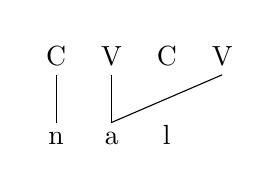
\begin{tikzpicture} 
\matrix [matrix of nodes, row sep=0.5em, 
         column sep={1em,between origins}, 
         row 5/.style={font=\scshape}] 
%
{ 
|(c1)| C    & & |(v1)| V                && |(c2)| C && |(v2)| V \\ [1em] 
|(n)| n  & & |(a)| a && |(l)| l \\
}; 


\draw (c1.south) -- (n.north); 
\draw (v1.south) -- (a.north); 
\draw (v2.south) -- (a.north); 
%
\end{tikzpicture}} \jambox{(\citealt{schiffman1999reference}:6)}

\end{xlist}
\end{exe}

\begin{exe}
\ex \label{new13}
\begin{xlist}
\ex \label{new13a}
maram   \hspace{2cm} 	[marõ]  \hspace{2cm}	'tree' 

\ex \label{new13b}
{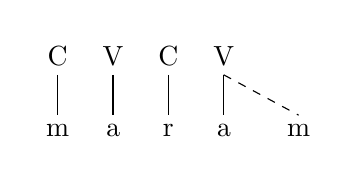
\begin{tikzpicture} 
\matrix [matrix of nodes, row sep=0.5em, 
         column sep={1em,between origins}, 
         row 5/.style={font=\scshape}] 
%
{ 
|(c1)| C    & & |(v1)| V                && |(c2)| C && |(v2)| V \\ [1em] 
|(m)| m  & & |(a)| a && |(r)| r && |(a2)| a && |(m2)| m \\
}; 


\draw (c1.south) -- (m.north); 
\draw (v1.south) -- (a.north); 
\draw (c2.south) -- (r.north); 
\draw (v2.south) -- (a2.north); 
\draw[dashed] (v2.south) -- (m2.north);
%
\end{tikzpicture}} \jambox{(\citealt{schiffman1999reference}:4)}

\end{xlist}
\end{exe}

The final /n/ of the pronominal \textsc{base}s in question in the previous section also floats. For example, in isolation \textit{naan} is pronounced [nãã] and \textit{en} is pronounced [yẽ] (\citealt{schiffman1999reference}:5). The onglide in the latter is predictable for initial mid-vowels.

The morphological breakdown in Section 2 brought us to the conclusion that the pronominal \textsc{base} alternations are not between \textit{naan/nii} and \textit{en/on}, but rather between \textit{n/en} in the 1$^{st}$ person, and \textit{n/on} in the 2$^{nd}$ person. It is fairly straightforward to conclude that the \textit{n} in each is the same consonant, and therefore has the same underlying representation \footnote{Tome Leu (p.c.) suggests that perhaps it is even the same morpheme, indicating ‘participant’.}.  From the pronunciation of \textit{en} in isolation (and of the 2$^{nd}$ oblique form in (\ref{new15b}) below) we can also conclude that this n is underlyingly floating. It is only pronounced when followed by a vowel. What, then, can we say about the \textit{e} of \textit{en} and the \textit{o} of on? We can suggest that these vowels too, are floating (the conditions for their pronunciation will be discussed further below), and that the underlying lexical entries for the \textsc{base} morpheme in the 1st and second person are as in (\ref{new14}). They contain no lexicalized structure on the CV-tier (compare the underlying structures with lexicalized CV structure in (\ref{new10c}), (\ref{new12b}), and (\ref{new13b})).

\begin{exe}
\ex \label{new14}
\begin{xlist}
\ex \label{new14a}
en	‘1\textsc{sg}’ 
\ex \label{new14b}
on	‘2\textsc{sg}’ 
\end{xlist}
\end{exe}

To explain the conditions under which the initial vowels of these \textsc{base} morphemes are pronounced, we can look first to their forms in isolation. The forms in (\ref{new14}) can be the overt manifestations of the oblique forms, whose suffix is null, with the pronunciations in (\ref{new15a},\ref{new15b}), and the nominative pronouns can be seen in (\ref{new15c},\ref{new15d}).

\begin{exe}
\ex \label{new15}
\begin{xlist}
\ex \label{new15a}
en-Ø 	\hspace{1cm}	‘\textsc{d}.1\textsc{sg-oblique}’	 \hspace{1.15cm}    	[$^{y}$ẽ]  \hspace{1cm}   	‘my’ 
\ex \label{new15b}
on-Ø 	\hspace{1cm}	‘\textsc{d}.2\textsc{sg-oblique}’	 \hspace{1cm}    	[wõ]   \hspace{0.95cm}    	‘your’ 
\ex \label{new15c}
en-een 	\hspace{0.7cm}    ‘\textsc{d}.1\textsc{sg-agr}’   \hspace{1.75cm} 		[nãã] \hspace{0.9cm}      	‘I’ 
\ex \label{new15d}
on-ii 	\hspace{1cm}	‘\textsc{d}.2\textsc{sg-agr}’      \hspace{1.75cm}    		[nii]   \hspace{1cm}     	‘you’ 
\end{xlist}
\end{exe}

Given that the /n/ of \textsc{base} is pronounced before the \textsc{agr} morphemes, we can assume that these morphemes come with lexicalized CV space, where \textit{een} has the underlying representation in (\ref{new16a}), and ii the underlying representation in (\ref{new16b}).

\begin{multicols}{2}
\begin{exe}
\ex \label{new16}
\begin{xlist}


\ex \label{new16a}
\begin{tikzpicture} 
\matrix [matrix of nodes, row sep=0.5em, 
         column sep={1em,between origins}, 
         row 5/.style={font=\scshape}] 
%
{ 
|(c1)| C    & & |(v1)| V                && |(c2)| C && |(v2)| V \\ [1em] 
|(m)|   & & |(a)|  && |(e)| e && |(a2)|  && |(n)| n \\
}; 


 
\draw (v1.south) -- (e.north); 
\draw (v2.south) -- (e.north); 
%
\end{tikzpicture}

\vfill \null
\columnbreak

\ex \label{new16b}
\begin{tikzpicture} 
\matrix [matrix of nodes, row sep=0.5em, 
         column sep={1em,between origins}, 
         row 5/.style={font=\scshape}] 
%
{ 
|(c1)| C    & & |(v1)| V                && |(c2)| C && |(v2)| V \\ [1em] 
|(m)|   & & |(a)|  && |(i)| i && |(a2)|   \\
}; 


 
\draw (v1.south) -- (i.north); 
\draw (v2.south) -- (i.north); 
%
\end{tikzpicture}
\end{xlist}
\end{exe}
\end{multicols} 

Each of the morphemes in (\ref{new16}) will allow for the syllabification of the /n/ of \textit{en} and \textit{on} as an onset. In other words, the syllabification of /n/ in (\ref{new14a}, \ref{new14b} ) will be enabled before the vowel-initial \textsc{agr} morphemes, as in (\ref{new17}). Remember that these \textsc{agr} morphemes do not appear in any pronominal forms except for the nominative. They are absent from all other cases. 

\begin{multicols}{3}
\begin{exe}
\ex \label{new17} 
\begin{tikzpicture} 
\matrix [matrix of nodes, row sep=0.5em, 
         column sep={0.5em,between origins}, 
         row 5/.style={font=\scshape}] 
%
{ 
|(e1)|     & & |(e2)|     & & |(e3)|     & & |(c1)| C    & & |(v1)| V                && |(c2)| C && |(v2)| V \\ [1em]  
|(e)| e  & &|(n)| n  & &|(dash)| -  & &|(m)|   & & |(m)|   & & |(e2)| e   && |(i)|  && |(n)| n   \\
}; 


 
\draw (v1.south) -- (e2.north); 
\draw (v2.south) -- (e2.north); 
%
\end{tikzpicture}

\vfill \null
\columnbreak
 {\textcolor{white}{.}} \\
\rightarrow 
 
\vfill \null
\columnbreak

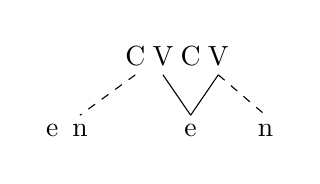
\begin{tikzpicture} 
\matrix [matrix of nodes, row sep=0.5em, 
         column sep={0.5em,between origins}, 
         row 5/.style={font=\scshape}] 
%
{ 
|(e1)|     & & |(e2)|     & & |(e3)|     & & |(c1)| C    & & |(v1)| V                && |(c2)| C && |(v2)| V \\ [1em] 
|(e)| e  & &|(n1)| n  & &|(dash)|   & &|(m)|   & & |(m)|   & & |(e2)| e   && |(i)|  && |(n2)| n   \\
}; 


 
\draw[dashed] (c1.south) -- (n1.north); 
\draw (v1.south) -- (e2.north); 
\draw (v2.south) -- (e2.north); 
\draw[dashed] (v2.south) -- (n2.north); 
%
\end{tikzpicture}

\end{exe}
\end{multicols}


In (\ref{new17}) the initial vowel is not pronounced, as the CV structure within the derivation provides no place for it to link. On the other hand, in all cases but the nominative we must explain why the initial vowels in \textit{en} and \textit{on} are pronounced. We cannot propose that the BASE morpheme is spelled out with its suffixes in these cases, as sometimes these suffixes also begin with a vowel, and should therefore allow for the same phonological analysis/predictions as in (\ref{new17}). A derivation for, say, the Accusative Singular [ennai] along the lines of (\ref{new17}) would erroneously predict the non-pronunciation of the initial vowel of the \textsc{base}.

\begin{multicols}{3}
\begin{exe}
\ex \label{new18} *
\begin{tikzpicture} 
\matrix [matrix of nodes, row sep=0.5em, 
         column sep={0.5em,between origins}, 
         row 5/.style={font=\scshape}] 
%
{ 
|(e1)|     & & |(e2)|     & & |(e3)|     & & |(c1)| C    & & |(v1)| V                && |(c2)| C && |(v2)| V \\ [1em]  
|(e)| e  & &|(n)| n  & &|(dash)| -  & &|(m)|   & & |(a)| a  & & |(e)|   & & |(i)| i  \\
}; 


 
\draw (v1.south) -- (a.north); 
\draw (v2.south) -- (i.north); 
%
\end{tikzpicture}

\vfill \null
\columnbreak
 {\textcolor{white}{.}} \\
\rightarrow 
 
\vfill \null
\columnbreak

\begin{tikzpicture} 
\matrix [matrix of nodes, row sep=0.5em, 
         column sep={0.5em,between origins}, 
         row 5/.style={font=\scshape}] 
%
{ 
|(e1)|     & & |(e2)|     & & |(e3)|     & & |(c1)| C    & & |(v1)| V                && |(c2)| C && |(v2)| V \\ [1em] 
|(e)| e  & &|(n1)| n  & &|(dash)| & & |(e)|     & &|(a)| a  & & |(m)|   & & |(i)| i  \\
}; 


 
\draw (v1.south) -- (a.north); 
\draw (v2.south) -- (i.north); 

%
\end{tikzpicture}

\end{exe}
\end{multicols}

Note also that the initial vowels and the nasals are pronounced in the Exclusive Plural forms, wherein the \textsc{base} morpheme is followed by a C-initial morpheme. This is also unexplained if the morphemes of the Exclusive Plural are interpreted together. (\ref{new19}) shows this predicted, and ungrammatical, derivation of the Exclusive Plural Accusative. Here the \textsc{base} is unlinked to the CV tier, and therefore remains unpronounced. The variable initial nasal of the plural morpheme is omitted here for ease of exposition.

\begin{multicols}{3}
\begin{exe}
\ex \label{new19} *
\begin{tikzpicture} 
\matrix [matrix of nodes, row sep=0.5em, 
         column sep={0.5em,between origins}, 
         row 5/.style={font=\scshape}] 
%
{ 
|(e1)|     & & |(e2)|     & & |(e3)|     & & |(c1)| C    & & |(v1)| V                && |(c2)| C && |(v2)|  V  & & |(e3)| & & |(c3)| C    & & |(v3)| V                && |(c4)| C && |(v4)| V \\ [1em]  
|(e)| e  & &|(n)| n  & &|(dash)| -  & &|(k)| k  & & |(a)| a  & & |(l)| ɭ  & & |(em)|  & & |(dash2)| - & & |(em)| & & |(a2)| a & & |(em)| & & |(i)| i     \\
}; 


 

\draw   (c1.south) -- (k.north); 
\draw (v1.south) -- (a.north); 
\draw (c2.south) -- (l.north); 
\draw (v3.south) -- (a2.north); 
\draw (v4.south) -- (i.north); 
%
\end{tikzpicture}

\vfill \null
\columnbreak
 {\textcolor{white}{.}} \\
\rightarrow 
 
\vfill \null
\columnbreak

*[kaɭai]

\end{exe}
\end{multicols}

We are left with but one possible analysis of the pronunciation of \textsc{base} in all of the pronominal forms that do not contain the \textsc{agr} morpheme. In these derivations, the pronominal root must undergo Spell Out in a cycle that does not include any of its suffixes. Before I can explain why this is the correct analysis of these pronominal forms, we must examine one further aspect of Tamil phonology. 

First, consider again example (\ref{new12}), where underlying /naal/ ‘day’ may surface as either  [naalʉ] or [naa], depending on the dialect. Now consider what must be occurring in the phonology in the derivation of a form like [naalʉ] under the lexico-structural assumptions laid out above. The final sonorant is unpronounced unless ‘saved’ by either the insertion of an epenthetic vowel, or by the syllabification of the final sonorant as the onset of a following word/morpheme, as for [aval] in (\ref{new20}).

\begin{exe}
\ex \label{new20}
\begin{xlist}
\ex \label{new20a}
ava pooraa	\hspace{1.8cm}	'she goes.' 
\ex \label{new20b}
aval-ukku 	\hspace{2cm}	‘to her' 
\end{xlist}
\end{exe}

In Tamil, the motivation for the epenthesis of the final vowel in [naalʉ] appears to be related to word-minimality. Word-minimality is a common cross-linguistic requirement that lexical words be bi-moraic or bi-syllabic \footnote{  For example, consider that English monosyllabic words may end in a long vowel (i), or a vowel-consonant (ii) (heavy, bi-moraic syllables), but monomoraic single-syllable words are disallowed (iii). 

(i)	bee [bii]	\hspace{1cm}	(ii) 	bit [bɪt]	\hspace{1cm}	(iii)	*[bɪ])

} .  Single-syllable words will undergo this epenthesis, while longer words are more likely to drop the final C. If the final C were not floating, we would expect it to always be pronounced. Since it is variably pronounced, we must assume that the epenthetic vowel affords it an onset position in which it may be syllabified. In CVCV phonology, every V position on the CV-tier comes with a preceding C (CV-sequences are the only units on the skeletal tier). Therefore, the V position in which the epenthetic vowel is pronounced will provide a consonantal position to which the final floating consonant may link. 

\begin{multicols}{5}
\begin{exe}
\ex \label{new21} 

\begin{tikzpicture} 
\matrix [matrix of nodes, row sep=0.5em, 
         column sep={0.5em,between origins}, 
         row 5/.style={font=\scshape}] 
%
{ 
|(c1)| C    & & |(v1)| V                && |(c2)| C && |(v2)| V \\ [1em]  
|(n)| n  & &|(em)|   & &|(a)| a  & &|(em)|   & & |(l)| l  \\
}; 


\draw (c1.south) -- (n.north); 
\draw (v1.south) -- (a.north); 
\draw (v2.south) -- (a.north); 
%
\end{tikzpicture}

\vfill \null
\columnbreak
 {\textcolor{white}{.}} \\
\rightarrow 
 
\vfill \null
\columnbreak


\begin{tikzpicture} 
\matrix [matrix of nodes, row sep=0.5em, 
         column sep={0.5em,between origins}, 
         row 5/.style={font=\scshape}] 
%
{ 
|(c1)| C    & & |(v1)| V    && |(c2)| C && |(v2)| V && |(em)| && |(c3)| C && |(v3)| V \\ [1em]  
|(n)| n  & &|(em)|   & &|(a)| a  & &|(em)|   & & |(l)| l  \\
}; 


\draw (c1.south) -- (n.north); 
\draw (v1.south) -- (a.north); 
\draw (v2.south) -- (a.north); 

%
\end{tikzpicture}

\vfill \null
\columnbreak
 {\textcolor{white}{.}} \\
\rightarrow 
 
\vfill \null
\columnbreak

\begin{tikzpicture} 
\matrix [matrix of nodes, row sep=0.5em, 
         column sep={0.5em,between origins}, 
         row 5/.style={font=\scshape}] 
%
{ 
|(c1)| C    & & |(v1)| V  && |(c2)| C && |(v2)| V && |(em)| && |(c3)| C && |(v3)| V \\ [1em]  
|(n)| n  & &|(em)|   & &|(a)| a  & &|(em)|   & & |(l)| l   & & |(em)|   & & |(u)| ʉ \\
}; 


\draw (c1.south) -- (n.north); 
\draw (v1.south) -- (a.north); 
\draw (v2.south) -- (a.north); 
\draw[dashed] (c3.south) -- (l.north); 
\draw (v3.south) -- (u.north); 

%
\end{tikzpicture}

\end{exe}
\end{multicols}

We can assume here that this epenthetic CV is not inserted except in cases where the underlying form is deemed too small, and that the pronunciation of the vocalic position is the default pronunciation of final empty vocalic positions in Tamil (in other words, the insertion of the epenthetic vowel is effected after the insertion of the CV augment; it is not underlyingly attached to the V position) \footnote{Note that word minimality requirements appear to be variable across dialects. I assume here that word-minimality repairs may be triggered if the underlying form contains only a single melodic vowel.}.  Now consider a derivation where the non-nominative pronouns are interpreted in two phonological cycles; one cycle that includes the BASE, and a second that includes the pronominal suffixes. 

If the \textsc{base} in the non-nominative pronominal derivations undergoes Spell Out alone in its cycle, and if our analysis of its underlying structure is correct, then word-minimality requirements will impose the insertion of this epenthetic CV space at PF in these derivations \footnote{Initial glides are predictable word-initially, and are coherent with the CVCV framework, or any phonological framework that favours the pronunciation of empty onset positions.}.  (\ref{new22}) shows the derivation of (\ref{new15a}), the D.1\textsc{sg-oblique} ‘my’. Here the derivation is effected in 2 steps. (\ref{new22a}) represents the output of cyclic phonology, where CV-slots are linked with melody from right to left. (\ref{new22b}) represents the output of post-cyclic phonology, where additional floating segments link to the CV tier in Tamil. That these two steps are distinct can be seen in the derivation of forms like \textit{ennai} (\ref{new23}).

\begin{exe}
\ex \label{new22}
\begin{xlist}

\ex \label{new22a}
\begin{multicols}{6}
\begin{tikzpicture} 
\matrix [matrix of nodes, row sep=0.5em, 
         column sep={0.5em,between origins}, 
         row 5/.style={font=\scshape}] 
%
{ 
|(c1)|     & & |(v1)|                 && |(c2)|  && |(v2)|  \\ [1em]  
|(em)|   & &|(e)| e  & &|(n)| n  \\
}; 


%
\end{tikzpicture}

\vfill \null
\columnbreak
 {\textcolor{white}{.}} \\
\rightarrow 
 
\vfill \null
\columnbreak

\begin{tikzpicture} 
\matrix [matrix of nodes, row sep=0.5em, 
         column sep={0.5em,between origins}, 
         row 5/.style={font=\scshape}] 
%
{ 
|(c1)|     & & |(v1)|     && |(c2)| C && |(v2)| V \\ [1em]  
|(e)| e  & &|(n)| n  & &|(em)|   & &|(em)|    \\
}; 



%
\end{tikzpicture}

\vfill \null
\columnbreak
 {\textcolor{white}{.}} \\
\rightarrow 
 
\vfill \null
\columnbreak

\begin{tikzpicture} 
\matrix [matrix of nodes, row sep=0.5em, 
         column sep={0.5em,between origins}, 
         row 5/.style={font=\scshape}] 
%
{ 
|(c1)|     & & |(v1)|     && |(c2)| C && |(v2)| V \\ [1em]  
|(e)| e  & &|(n)| n  & &|(em)|   & &|(em)|    \\
}; 


]
\draw[dashed] (v2.south) -- (e.north); 
]
%
\end{tikzpicture}

\vfill \null
\columnbreak
 {\textcolor{white}{.}} \\
 {\textcolor{white}{...}}[e]  

\end{multicols}


\ex \label{new22b} 
\begin{multicols}{6}
\begin{tikzpicture} 
\matrix [matrix of nodes, row sep=0.5em, 
         column sep={0.5em,between origins}, 
         row 5/.style={font=\scshape}] 
%
{ 
|(c1)|     & & |(v1)|                 && |(c2)|  && |(v2)|  \\ [1em]  
|(em)|   & &|(e)| e  & &|(n)| n  \\
}; 


%
\end{tikzpicture}

\vfill \null
\columnbreak
 {\textcolor{white}{.}} \\
\rightarrow 
 
\vfill \null
\columnbreak

\begin{tikzpicture} 
\matrix [matrix of nodes, row sep=0.5em, 
         column sep={0.5em,between origins}, 
         row 5/.style={font=\scshape}] 
%
{ 
|(c1)|     & & |(v1)|     && |(c2)| C && |(v2)| V \\ [1em]  
|(e)| e  & &|(n)| n  & &|(em)|   & &|(em)|    \\
}; 



%
\end{tikzpicture}

\vfill \null
\columnbreak
 {\textcolor{white}{.}} \\
\rightarrow 
 
\vfill \null
\columnbreak

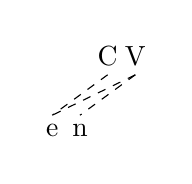
\begin{tikzpicture} 
\matrix [matrix of nodes, row sep=0.5em, 
         column sep={0.5em,between origins}, 
         row 5/.style={font=\scshape}] 
%
{ 
|(c1)|     & & |(v1)|     && |(c2)| C && |(v2)| V \\ [1em]  
|(e)| e  & &|(n)| n  & &|(em)|   & &|(em)|    \\
}; 


]
\draw[dashed] (v2.south) -- (e.north); 
\draw[dashed] (v2.south) -- (n.north); 
\draw[dashed] (c2.south) -- (e.north); 


]
%
\end{tikzpicture}

\vfill \null
\columnbreak
 {\textcolor{white}{.}} \\
 {\textcolor{white}{...}} [$^y$ẽ]  

\end{multicols}


\end{xlist}
\end{exe}

Before going on to (\ref{new23}), note that this analysis has the added advantage of offering an account of a discrepancy between the pronunciation of pronouns like \textit{en} and single syllable lexical items like \textit{naal} ‘day’. If lexical items like \textit{naal} have underlying CV structure linked to all melodic elements, save for the final floating consonants (the standard assumption for non-alternating phonological forms), then an epenthetic CV will offer space for the pronunciation of this floating consonant. In the case of \textit{en}, however, the CV cannot provide for the attachment of /n/ to the C position without crossing autosegmental lines. The only option is therefore to link the nasal to the vocalic position. Final Cs in function words and final Cs in lexical words are therefore predicted to behave distinctly in the presence of an epenthetic CV, as is the case.

In the derivation of an overtly morphologically complex form like [ennai] the derivation in (\ref{new22a}) will be the output of a first cycle of interpretation. In the second cycle the affixation of \textit{ai} will offer a position for the pronunciation of [n], as in (\ref{new23}). Post-cyclic nasalization of the vowel of the \textsc{base} will not occur, as [n] has linked to a C-position, while post-cyclic ongliding will still occur. Recall that we have put aside the question of how gemination is derived here (see footnote 3).

\begin{multicols}{4}
\begin{exe}
\ex \label{new23} 
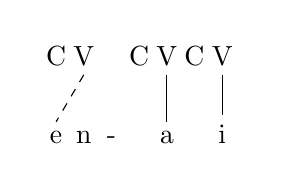
\begin{tikzpicture} 
\matrix [matrix of nodes, row sep=0.5em, 
         column sep={0.5em,between origins}, 
         row 5/.style={font=\scshape}] 
%
{ 
 |(c1)| C    & & |(v1)| V & &  |(e1)|    && |(c2)| C && |(v2)| V   && |(c3)| C    & & |(v3)| V    & & \\ [1em]  
|(e)| e  & &|(n)| n  & &|(dash)| -  & &|(em)|   & & |(a)| a  & & |(em)|   & & |(i)| i  \\
}; 


\draw[dashed] (v1.south) -- (e.north); 
\draw (v2.south) -- (a.north); 
\draw (v3.south) -- (i.north); 
%
\end{tikzpicture}

\vfill \null
\columnbreak
 {\textcolor{white}{.}} \\
\rightarrow 
 
\vfill \null
\columnbreak

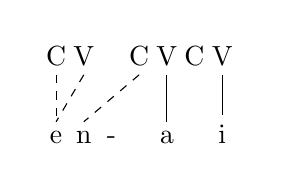
\begin{tikzpicture} 
\matrix [matrix of nodes, row sep=0.5em, 
         column sep={0.5em,between origins}, 
         row 5/.style={font=\scshape}] 
%
{ 
|(c1)| C    & & |(v1)| V  & &  |(e1)|        && |(c2)| C && |(v2)| V  && |(c3)| C    & & |(v3)| V    & & \\ [1em]  
|(e)| e  & &|(n)| n  & &|(dash)| -  & &|(em)|   & & |(a)| a  & & |(em)|   & & |(i)| i  \\
}; 


 
\draw[dashed] (c1.south) -- (e.north); 
\draw[dashed] (v1.south) -- (e.north); 
\draw[dashed] (c2.south) -- (n.north); 
\draw (v2.south) -- (a.north); 
\draw (v3.south) -- (i.north); 

%
\end{tikzpicture}

\vfill \null
\columnbreak
 {\textcolor{white}{.}} \\
 {\textcolor{white}{...}} [$^y$ennai]

\end{exe}
\end{multicols}

\section{Possible syntactic motivations for the bi-cyclic analysis}

The analysis above makes specific predictions about the cyclic Spell Out domains in the morphosyntax of the Tamil pronominal system. It is proposed that in all derivations but the nominative, the pronominal \textsc{base} undergoes Vocabulary Insertion in its own cycle,  alone. In the following paragraphs I suggest some syntactic paths to follow that would support the proposed phonological analysis in Section 3. 

One option is that there is a cyclic domain that triggers PF interpretation of the root in the derivation of all pronouns (the \textsc{base} is interpreted separately from the \textsc{pl/k}(ase) heads in all derivations) but that there is an operation of agreement that is triggered only when the pronoun is nominative. This domain is labeled F in (\ref{new24}).

\begin{exe}

\ex \label{new24}
\begin{xlist}
\begin{multicols}{2}
\ex \label{new24a}
%24a 
\begin{forest}
[K(ase)
[(PL)
[AGR
[\textbf{BASE} \\ \textbf{en/on}][\textbf{Ø+AGR}]
][(n)kaɭ]
][NOM\\ Ø]
]
\end{forest}

\vfill \null
\columnbreak

\ex \label{new24b}
%24b
\begin{forest}
[K(ase)
[(PL)
[AGR
[\textbf{BASE} \\ \textbf{en/on}][\textbf{Ø}]
][(n)kaɭ]
][NOM\\ Ø]
]
\end{forest}
\end{multicols}

\ex \label{new24c}
Spell-Out of \textsc{\textbf{f}} in (\ref{new24a}) \rightarrow \hspace{0.1cm} (i) VI of \textsc{base} : /en/~/on/ \\
 \textcolor{white}{ooooooooooooooooooooo} (ii) VI of dissociated \textsc{agr} :/aan/ \\
 \textcolor{white}{ooooooooooooooooooooo} (iii) Phonological derivation as in (\ref{new17}) \\
Spell-Out of \textsc{\textbf{k}} in (\ref{new24a}) \rightarrow \hspace{0.1cm} (i) VI of K and PL : /(n)kaɭ/ \\
 \textcolor{white}{ooooooooooooooooooooo}   (ii) Linearization of BASE+ PL \\
 \textcolor{white}{ooooooooooooooooooooo}  (iii) Phonological derivation of [naaŋkaɭ]
\ex \label{new24d}
Spell-Out of \textsc{\textbf{f}} in (\ref{new24b}) \rightarrow \hspace{0.1cm} (i) VI of \textsc{base} : /en/~/on/ \\
 \textcolor{white}{ooooooooooooooooooooo} Phonological derivation as in (\ref{new22a}) \\
 Spell-Out of \textsc{\textbf{k}} in (\ref{new24b})  \rightarrow \hspace{0.1cm} (i) VI of K and PL : /(n)kaɭ/ + /ai/ \\
 \textcolor{white}{ooooooooooooooooooooo} 	(ii) Linearization of BASE+ PL+K \\
  \textcolor{white}{ooooooooooooooooooooo}	(iii) Phonological derivation of [eŋkaɭai] 
\end{xlist}
\end{exe}

This analysis clearly assumes that the nominative head is present in the structure before \textsc{\textbf{f}} is spelled out in (\ref{new24}), as \textsc{\textbf{f}} must only trigger the insertion of \textsc{agr} in the scope of nominative case. In phase theory spell-out of a phase (here \textsc{\textbf{f}}) may be triggered by the merger of a higher phase head (here K, or a higher functional head in the pronominal structure), allowing for agreement of \textsc{\textbf{f}} and \textsc{\textbf{nom}} prior to PF interpretation of \textsc{\textbf{f}}. If the agreement morphemes attached to F are dissociated (à la \citealt{Embick1997}), then these morphemes will be inserted post-syntactically. In this analysis the \textsc{agr} head is not present in the narrow syntax, and the derivations diverge at Vocabulary Insertion (VI), as in (\ref{new24c}, \ref{new24d}). 

A second option is that, instead of the difference between the presence of \textsc{agr} in the nominative, and its absence in all other cases, there is a different distinction that triggers the extraction of BASE to a specifier position in all cases/\textsc{k}(ase)s but the nominative. This type of account would entail that, for example, some feature in \textsc{k} attracts the root to its specifier, and this feature is present only in structures larger than the nominative. For expository purposes, the nominative in (\ref{new25})  is represented as \textsc{k}1, and \textsc{k}1+n refers to all case structures that are larger than the nominative.

\begin{exe}

\ex \label{new25}
\begin{xlist}
\begin{multicols}{2}
\ex \label{new25a}
%24a 
\begin{forest}
[K(ase)1
[(PL)
[AGR
[BASE \\ en/on][een-ii]
][(n)kaɭ]
][NOM\\ Ø]
]
\end{forest}

\vfill \null
\columnbreak

\ex \label{new25b}
%25b
\begin{forest}
[K1+n
[BASE \\ en/on,name=base2]
[K1+n
[(PL)
[\textcolor{gray}{\sout{(AGR)}}
[\textcolor{gray}{BASE} \\ \textcolor{gray}{en/on},name=base][\textcolor{gray}{\sout{een-ii}}]
][(n)kaɭ]
][NOM\\ Ø]
]]
\draw[->] (base) to[out=north west,in=south west] (base2);
\end{forest}
\end{multicols}



\ex \label{new25c}
Spell-Out of (\ref{new25a} = K1)  \rightarrow \hspace{0.1cm} (i) VI, linearization of \textsc{base}, \textsc{k} and \textsc{pl}  \\
 \textcolor{white}{oooooooooooooooooooooo} (ii) PPhonological derivation of ex. [naaŋkaɭ] 
 \textcolor{white}{ooooooooooooooooooo.oo} in a single cycle.



\ex \label{new25d} 
Spell-Out of \textsc{base} in (\ref{new25b}) \rightarrow \hspace{0.1cm} (i) Spell-Out of moved \textsc{base} 	Derivation \textcolor{white}{oooooooooooooo.oooooooooo} is identical to Spell-Out 	of \textbf{\textsc{f}} in (\ref{new24b})


	Spell-Out of K1+n in (\ref{new25b})  \rightarrow \hspace{0.1cm} (i)Derivation is identical to Spell-Out of  \textcolor{white}{oooooooooooooooooo.oooooo} \textsc{k} in (\ref{new24b})\footnote{  Laura Kalin, p.c., notes that this second derivation appears to be incompatible with an eventual analysis of the 1PL inclusive along the lines presented herein, where we would want the BASE to spell out with its suffix regardless of Kase.}
\end{xlist}
\end{exe}

In the Spell-Out of (\ref{new25a}) we have, following \citet{Moskal2015} and \citet{moskal2016towards}, a single cycle of interpretation at the \textsc{k}1 node. The form of the \textsc{base} falls out of the phonological analysis in Section 3. In the Spell-Out of (\ref{new25b}), we again have a cycle of Spell-Out triggered at the topmost \textsc{k}1+n node. But, in addition to this, we have a movement operation of the \textsc{base} to the Specifier of the \textsc{k}1+n projection. Following \citet{Johnson2004} and other work on the phonological interpretation of specifiers/left-branches, the \textsc{base} will be interpreted separately from the structure to which it is copy-merged. In this separate cycle, the phonological analysis in Section 3 applies to the \textsc{base}, and the linearization/spell-out of the heads within K1+n will be determined separately. \textsc{\sout{agr}} in (\ref{new25b}) is not inserted. It may either be absent, or it may fail to be inserted in any derivation where the \textsc{base} raises out of its scope. Note that if \citet{mcfadden2018aba} is correct and there is no nominative case head in the syntax, it becomes easier to distinguish why the \textsc{base} is attracted to the specifier only in derivations where there is a K(ase) projection.

Either of the above accounts would allow for the phonological analysis in Section 3 to explain the alternations between \textit{en/on} and \textit{n} in the Tamil pronominal paradigm without requiring any complication to the analysis of adjacency for suppletion cross-linguistically. Should derivations like in (\ref{new24}) and (\ref{new25}) be clearly impossible accounts for the data, the phonological analysis would then be improbable, and the complications raised for suppletion by the Tamil facts would again stand.

\section{Conclusions}

In the previous sections I have laid out arguments for an analysis that offers an alternative to the account in \citet{Moskal2015} and \citet{moskal2016towards} of Tamil pronominal alternations. These works have proposed that Tamil is a particular (although not the only) argument against a strict-adjacency (either structural or linear) account of suppletion, as suppletion is triggered across the plural morpheme. If, however, the phonological evidence is to be believed, this example is not a case of suppletion at all, but rather falls out of the regular derivational and representational phonology of the language (admitting that the relevant vowel quality alternations and gemination are still to be accounted for). If this egregious example of anti-locality is removed from the discourse on suppletion, one wonders if the other less fraught examples might also have alternative explanations. It is, of course, not the case that all of the patterns problematic for adjacency have phonological solutions. The  problems evoked by the pruning operation (\citealt{Embick2003}, \citeyear{embick2010localism}) discussed by \citet{Moskal2015} and \citet{moskal2016towards} are not (clearly) phonological issues, and accounts of allomorphy that appeal to Domain Suspension (\citealt{bobaljik2012universals}; \citealt{BobaljikWurmbrand2013}) or spanning (\citealt{Merchant2015}, \citet{svenonius2016spans}) clearly include cases where a morphosyntactic analysis must be appealed to (although, see \citet{newell2018re} for a teaser of a phonological analysis of the\textit{ de le} \rightarrow \textit{du} portmanteau problem in French). The analysis in Section 3 is just one alternative piece of the puzzle that may clear the way for a simpler explanation of locality restrictions in the domain of allomorphy.

Finally, I just want to situate this analysis in the larger setting, where questions of allomorphy and suppletion butt up against questions of phonological alternations. In either case, whether we posit suppletive forms or articulated phonological representations, the speaker must lexcialize something special about a particular vocabulary item. Whether we propose (seemingly small) complications to our phonological or to our morphosyntactic derivations leads to different predictions for the role of lexicalization and its effects on the linguistic system globally.

\section*{Abbreviations}
\begin{tabularx}{.45\textwidth}{lQ}
... & \\
... & \\
\end{tabularx}
\begin{tabularx}{.45\textwidth}{lQ}
... & \\
... & \\
\end{tabularx}

\section*{Acknowledgements}
I would like to thank two anonymous reviewers, as well as Tom Leu and Laura Kalin for helpful comments and discussions.

\printbibliography[heading=subbibliography,notkeyword=this]


\end{document}